\chapter{Methodology of Refactoring Process}


% % Application
% - Always with software system in mind
% - Methodological approach may vary depending on the software system at hand
% - For instance, the methodological approach design decisions that follow are made on the basis of the characteristics software system

\bigskip % Adds empty line
\begin{figure}[htp]
    \centering
    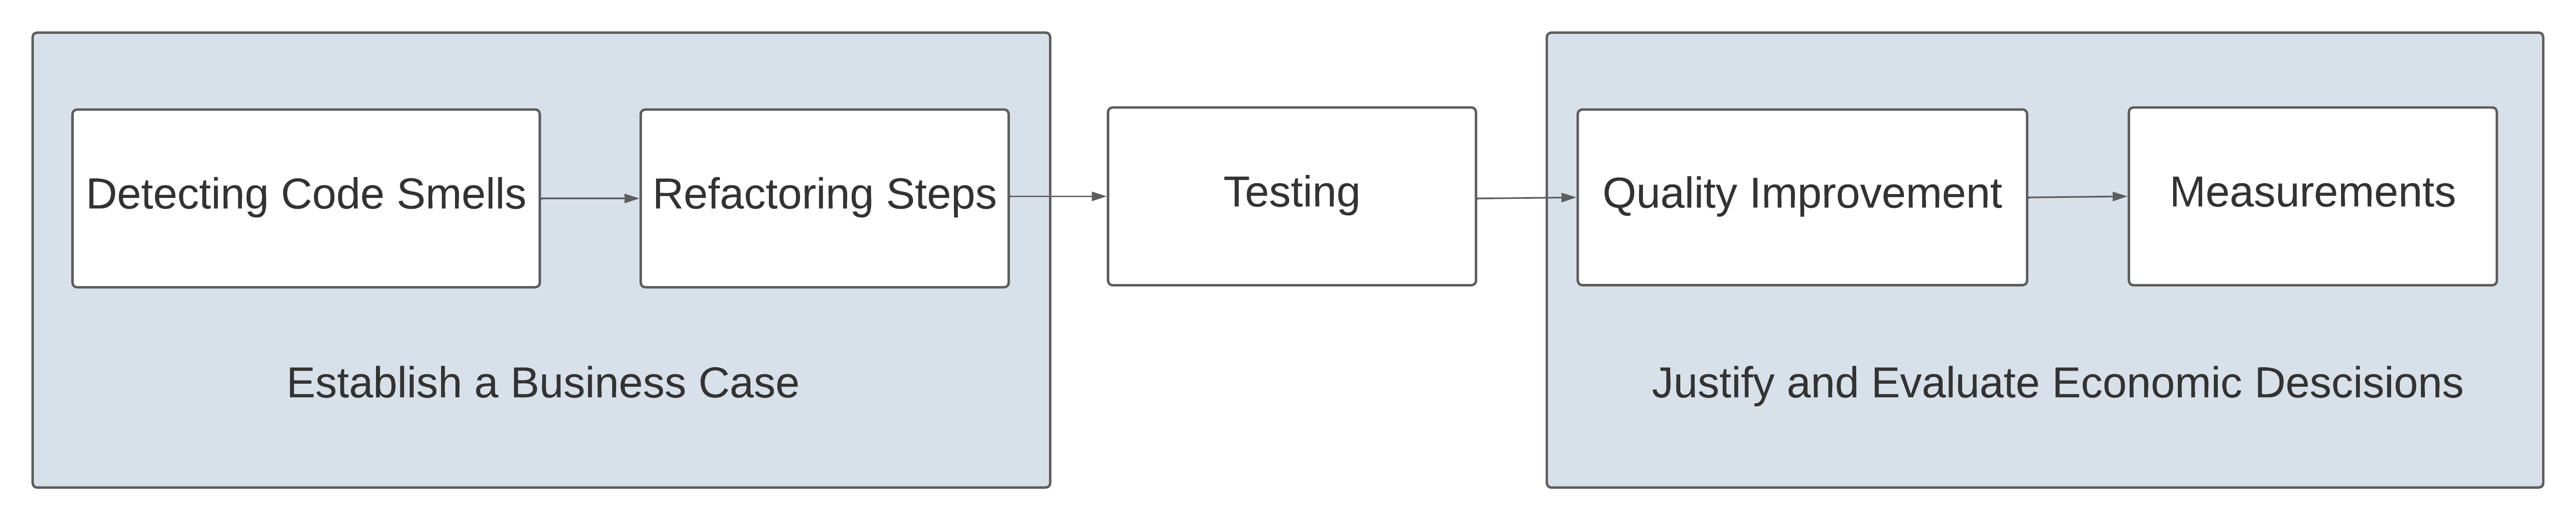
\includegraphics[width=\textwidth]{./assets/extended_refactoring}
    \caption{Extended model of Refactoring}
\end{figure}
\bigskip % Adds empty line

[Transition needed that introduces chapter with its contents]


[Also the model should be briefly described with its broader implications]

% Extension of the Refactoring process
% - In the end it should be clear, why refactoring is tightly integrated in other development processes
% - The above model summarizes the model that is used (-> The importance of why each stage is included will be explained in the corresponding chapters)
% - List this model; tell what is extra included
% - This will also be a hypothesis (That we can extend our refactoring; see where it connects to optimize it) -> There are no indications about this in literature, as far as concerned (verify)

% Short decription of each part of process
% -> Get an initial understanding


\section{Detecting Code Smells}

% Introduction Paragraph
The following part of this chapter moves on to describe in greater detail the detection of code smells within the software system. It provides a brief overview of the methods used and mentions the prevalence of the program \emph{Sonargraph} as the software tool used in the detection activities. Moreover, this section provides necessary clarifications to understand why certain methods were chosen over others.

% Catalogue
As previously stated, not all 24 code smells that are examined throughout Martin Fowler's book were used in the detection work. Instead, the 10 most frequently reported code smells have been chosen according to the work of \textcite{lacerda2020} %[p.~15]
Further, two additional smells \emph{refused bequest} and \emph{data clumps} were discarded. The decision was made due to their focus on inheritance and data structures respectively. More particular, these two programming abstractions are not utilized in the code, and are thus not of relevance in the detection. In order to revisit the code smell catalog with their corresponding explanation, refer to \ref{sec:smells}. Two primary reasons exist that have led to the decision of restricting the amount of smells for this section. First, it is not in the scope of the thesis to find each and every code smell in the codebase. The aim is rather to find the problems that are most apparent. Second, including more smells would be less of a problem, if automatic code detection tools could be used. Without being able to detect automatically, a limited amount of smell is more appropriate in order to not overspend time. A detection approach based on automatic tools is unfortunately not available for the python programming language, as will be alluded to in the section below. 

\subsection{Detection Methods}
% Metrics based
Many tools have been created to automatically or semi-automatically detect code smells (\cite{menshawy2021}). In the context of our thesis, the code smells are detected semi-automatically using a metric-based approach. This approach measures source code elements and takes decisions based on threshold values (\cite{menshawy2021}). It is fulfills two requirements necessary for the following work. On the one hand, it to a certain degree contains automation, increasing the efficiency and standardization in comparison to manual approaches. Further, it can be used for the python programming language, which is an essential prerequisite in the software system at hand. Menshawy additionally points out that a metrics approach does not provide metrics for every code smells. Nevertheless, for the eight smells the thesis is focussing on, as will be seen afterwards, an appropriate metric was found. 

[Personal Note: This can also be argued by lacerda's work, which states for all of these metrics a metric-based approach exists]

% Automation based
Using a detection approach utilizing automated tools would have been more attractive, but unfortunately not possible.  It is the most used approach (\cite{menshawy2021}), its availability is however highly dependent on the programming language the software system is written in (\cite{menshawy2021}). Further, looking at Menshawy's research on the most cited tools, it can be observed that a significant difference exists between java programming language, which was supported  by 48\% of the tools, whereas the python was supported by mere 4\%. In addition, by researching possible automated tools appropriate for python, it was evident that at this moment of time, the offering is insufficient to accomplish a comprehensive detection strategy. 

% Manual approach
In the beginning, the author also considered following a manual approach. In contrast to automation, the manual detection relies on human perception of smells by applying predefined guidelines (\cite{menshawy2021}). It is characterized as highly time-consuming and prone to human error. Therefore, when comparing this approach to a metrics-based, it is less desirable and was subsequently discarded as a detection technique.

% Visualization
Another detection approach that has not yet been mentioned, is the detection by means of code visualization. Although it only is used to detect a subset of smells, visualization provided to be of use in two occurrences throughout the thesis. First, it had been used to get a broad overview of the code base, which helped the author with orientation. Second, it was used to aid in judgments regarding coupling and cohesion of the code base. 

\subsection{Sonargraph}
% Intro Sonargraph
As indicated in the beginning of this chapter, the detection of code smells relied heavily on a code analyzer tool called Sonargraph. Its usage demonstrated to be extremely useful in the detection of code smells, by its ability to compute and list metrics of the software system. The software included sufficient and diverse selection of metrics. These metrics provided insights by both evaluating the entire project and also its individual modules. For each metric, Sonargraph offered explanations, which allowed for an appropriate metric to be found regarding each relevant code smell.

% Explorer + Metrics
Compared to other software solutions, Sonargraph was chosen for several reasons. Although the full suite of Sonargraph Applications is not free of charge, its graphical application \emph{Sonargraph Explorer} was free to use. For the thesis, it provided both numerical and visual methods to make observations about the code base. All the tools needed to compute metrics were accessible. Another noteworthy benefit of using Sonargraph during the detection, was its ability to observe the entire project,  and not just at individual files. This was essential for metrics taking account of dependencies between modules. In addition, it was beneficial not to rely on a multitude of software tools, by having just one software.

% Code duplicate
It is important to note that there was not an appropriate metric that could easily detect code duplication. However, in its paid version, accessible within a trial period, an automatic tool to detect code duplicates was provided.  Previously, it was stated that it was difficult to find automatic tools to detect code smells in a software system written in python. Duplicate code particularly differs from the other smells, as it can be detected language agnostic. In other words, to detect duplication of code in programs, the software does not need to understand the programming language. This same mechanism could theoretically be applied to other types of text that are not code. Surprisingly, the restriction of a trial period did not prove to be a problem. It was possible to renew a trial period multiple times, although this was not indicated on its website. As no guarantee can be given on the amount of reactivation, one must still be aware of this restriction. 

\subsection{Metrics Overview}

\begin{figure}[htp]
    \centering
    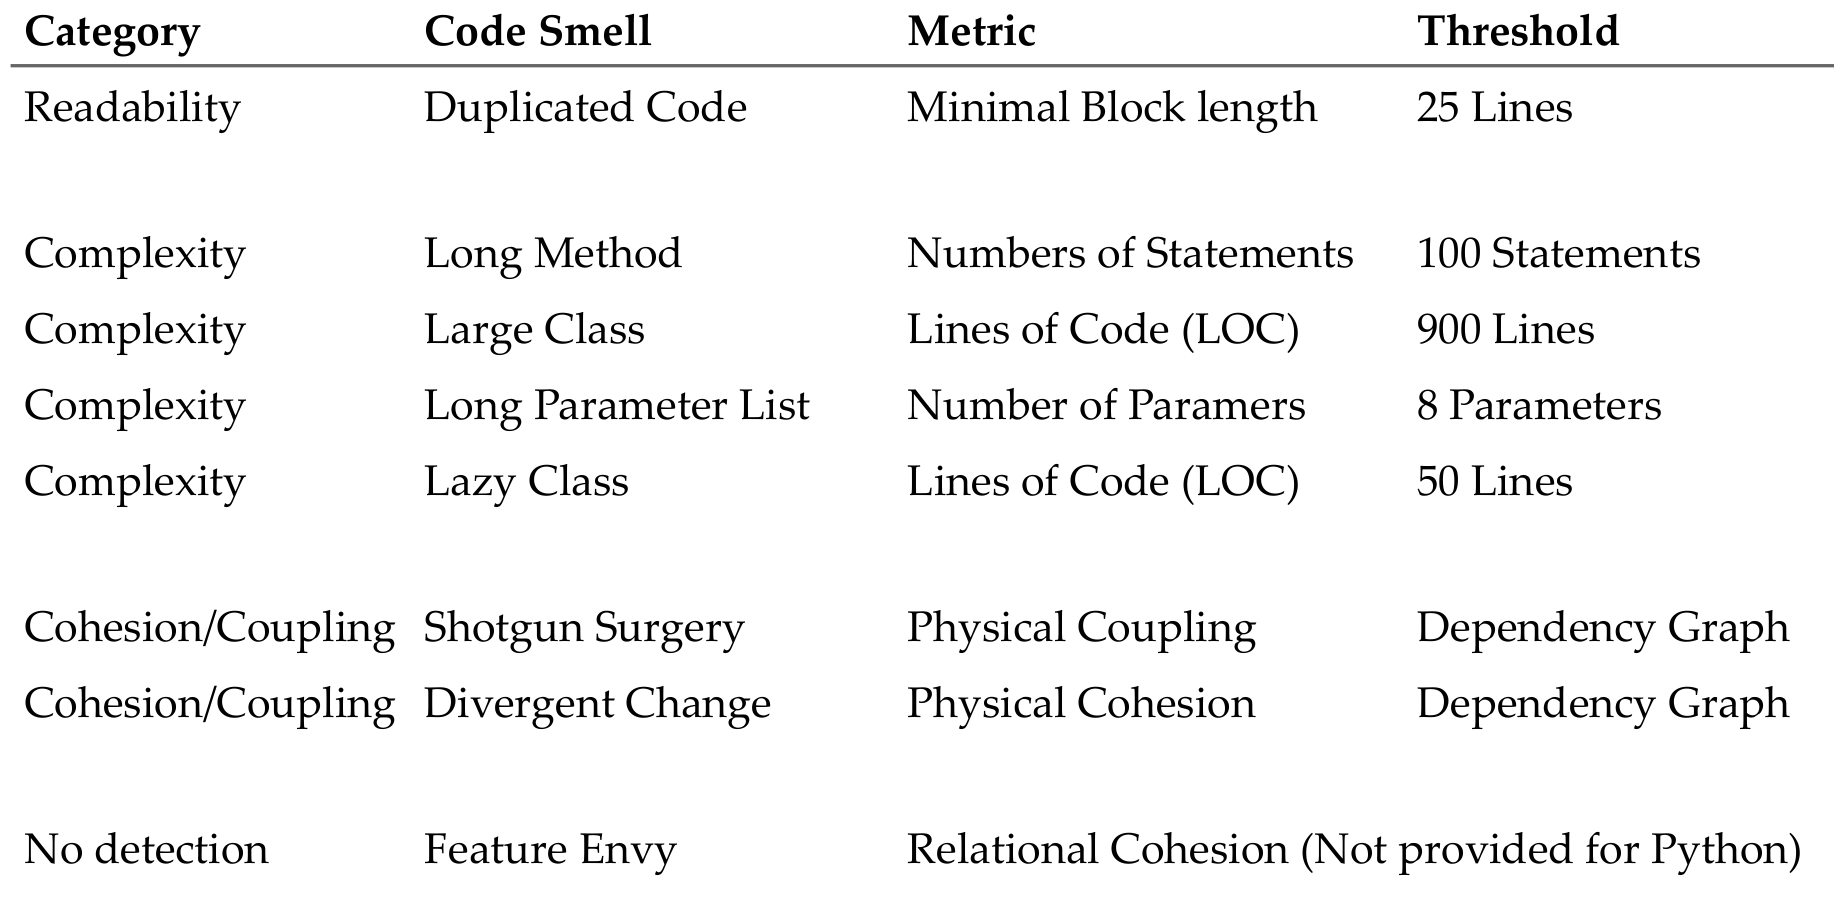
\includegraphics[width=\textwidth]{./assets/smell_overview}
    \caption{Metrics without prioritization}
\end{figure}
% Table
The above table presents for each code smell a corresponding metric. In addition, for some metrics, a threshold value is given. When the threshold value is surpassed, there is an indication that this code smell exists in the software system.

% Subgroups
Individual metrics are categorized into three subgroups, named after the quality attribute they best represent. More importantly, however, this distinction is made, as each of the group differs in regard to how a metric results in a smell detected. For example, as mentioned before, the subgroup readability differs considerably due to the fact that code duplication is automatically detected. In this case, the application limits the detection to a minimum of 25 Lines. This means that only duplicated are shown if they surpass this amount. 

% Complexity -> Threshold
Half of the code smells, in the subgroup called complexity, follow a typical metrics based approach. The threshold value indicate when a code smell is potentially present. Notably, all the metrics in this category involve counting of some sorts. In particular, the smells are detected by counting the number of statements, lines of codes, and numbers of parameters of methods. Prioritization of given smells can be done by comparing the extent of how much a given threshold value is surpassed. Similarly, code smells can be discarded if the associated metric does not surpass the threshold value. 

% Cohesion/Coupling -> Dependency graph
Lastly, Shotgun Surgery and Divergent change respectively are bound to the coupling and cohesion of the software system. The metric used measures the dependencies “to” and “from” other components, in either the same module (cohesion) or in other modules (coupling). The appropriate threshold value highly depends on the size of the software system. By adding code to the code base, we naturally increase the amount of expected dependencies. Therefore, the author decided to use incorporate a dependency graph in addition to the metrics, in order to evaluate the prominence of these two code smells.


\section{Testing}
% Transition
In the chapter that follows, the relevance of testing as a fundamental part of the refactoring process will be discussed. Subsequently, the challenges of testing a cyber physical system will be described. Based on these findings, the particular methods used for testing of the software system 
will be outlined at the end of this chapter.

\subsection{Importance of Testing in a Refactoring Process}

% Importance of Tests
Turning now to the importance of testing within the context of the refactoring process.  In order to understand the significance, it is appropriate to return to Martin Fowler's definition of refactoring (\cite{fowler2018}) as first discussed in section \ref{sec:background}. According to his definition, refactoring must not alter the external behavior of code. It was pointed out in the theoretical part of this thesis that by not changing the features of the program, programmers can alleviate the risks associated with changing the codebase, with the predominant focus of not introducing new bugs. As a result, to demonstrate that the behavior of the code base was not altered during refactoring, testing is necessary. Moreover, to confirm of an unaltered state of code behavior is vital to verify the improvement of code quality. Therefore, without testing we would get a false sense of an improvement of code quality, as potentially negative alterations are not taken into consideration. Hence, only with testing we can ensure that after refactoring the software system is in a better state than before.

\subsection{Testing Cyber Physical Systems}

% Transition
Knowing the benefits of testing, it is also important to discuss the challenges, granted that our software system is a cyber-physical system (CPS). These challenges arise due to the unique characteristics of a CPS and need to be taken into account when determining the methodology of testing these systems. 

% CPS Hetereogenous Nature
Robots and other cyber-physical systems react to information from the physical worlds and must operate safely even in the presence of uncertainties \cite{geissvolkermaria}. In such a dynamic real-world environment, \textcite{kapurpulkit2020} describes testing a CPS, as time-consuming and a particularly complicated task for developers. He points out that this is especially the case as it is difficult to ensure a robot will behave as expected. Similarly, \textcite{raikumar2010} point out the challenge of verifying and validating software systems due to their heterogeneous nature. Furthermore, it is hard to define the boundaries and physical limitations of the testing landscape made for a CPS (\cite{abbaspourasadollah2015}). 

% Automation
Another limitation in CPS testing is the introductions of automated semi-automated methods. Here, the efficacy of testing is limited by the element of its hardware components. Moreover, running tests is dependent on the hardware's capabilities, and that it is operating as expected. For instance, CPS with physical motions are subject to considerable time running tests and potentially require human supervision and manual intervention. Some of these challenges can be mitigated by using a physics-based simulation that mimics the real-world environment. (\cite{kapurpulkit2020}). Such solutions do exists in practice, but are unfortunately unavailable to our software system.

% Software test -> Manual test
This challenging physical environment of CPS ultimately results in programmers having to satisfy multiple levels when testing the software. The levels of CPS software testing contains verifying software, hardware, network, and the integration of all these components to work as a single system {abbaspourasadollah2015}. In general, there is a high interest to use automated testing, as manual testing is more likely to produce errors {turlea2019}. Despite automated tests having advantages such as more testing in less time and improvements in quality, it needs to be considered that no software tests are available for the software system at hand. In particular, the major disadvantages of automated tests are the costs associated with developing test automation, especially in dynamic customized environments (\cite{taipale2011}). Consequently, developing a testing suite having to develop a test suite from scratch forces us to choose a manual approach. It is important to note, that in future work, it would be appropriate to consider developing software tests. It is however not in the scope of this thesis to also take on this undertaking.

% One advantage
One advantage of the physical nature of CPS is that we are able to make visual observation. This feature can be viewed as a possible advantage in the manual testing of a particular CPS. Whether the observation of a CPS can be used in testing, is arguably strongly dependent on the type. In our case, there are no restrictions in observing the system visually. The benefits of such an approach become especially apparent when taking into account that our software project is focussing on managing entire processes. In more concrete terms, we are able to perceive visual changes in the behavior of our CPS by running a predefined process.  All in all, the lack of software tests and the ability to visually observe behavioral changes encouraged the decision to include manual testing,  as a preferred method. Even though this approach can not predict the equivalence of the entire software system, this method of testing can to a certain degree ensure no alterations within a particular processes. Moreover, this approach presumably inferior to comprehensive unit and integration testing. Nevertheless, it is an approach that suits the preconditions within our context, by determining changes within the scope of processes.

\subsection{Method selection}

% Transition
As just indicated, testing for this thesis will be done manually by means of observing an entire process of the CPS. To reduce the risks of uncertainty, methods are selected based on their ability to test objectively and in a routinized manner. To achieve this goal, two methods have been chosen, where one enables testing automation, while the other improves objectivity. In particular, the software application Camunda Modeler is used to automate the business processes and the Gherkin Language is used to objectively formulate requirements. In combination, these tools deliver a procedure to reduce ambiguity, which is a fundamental prerequisite when trying to capture any cue in observable changes. As a result, this approach reduces some shortcoming of manual testing, while also decreasing human error.

\begin{figure}[htp]
    \centering
    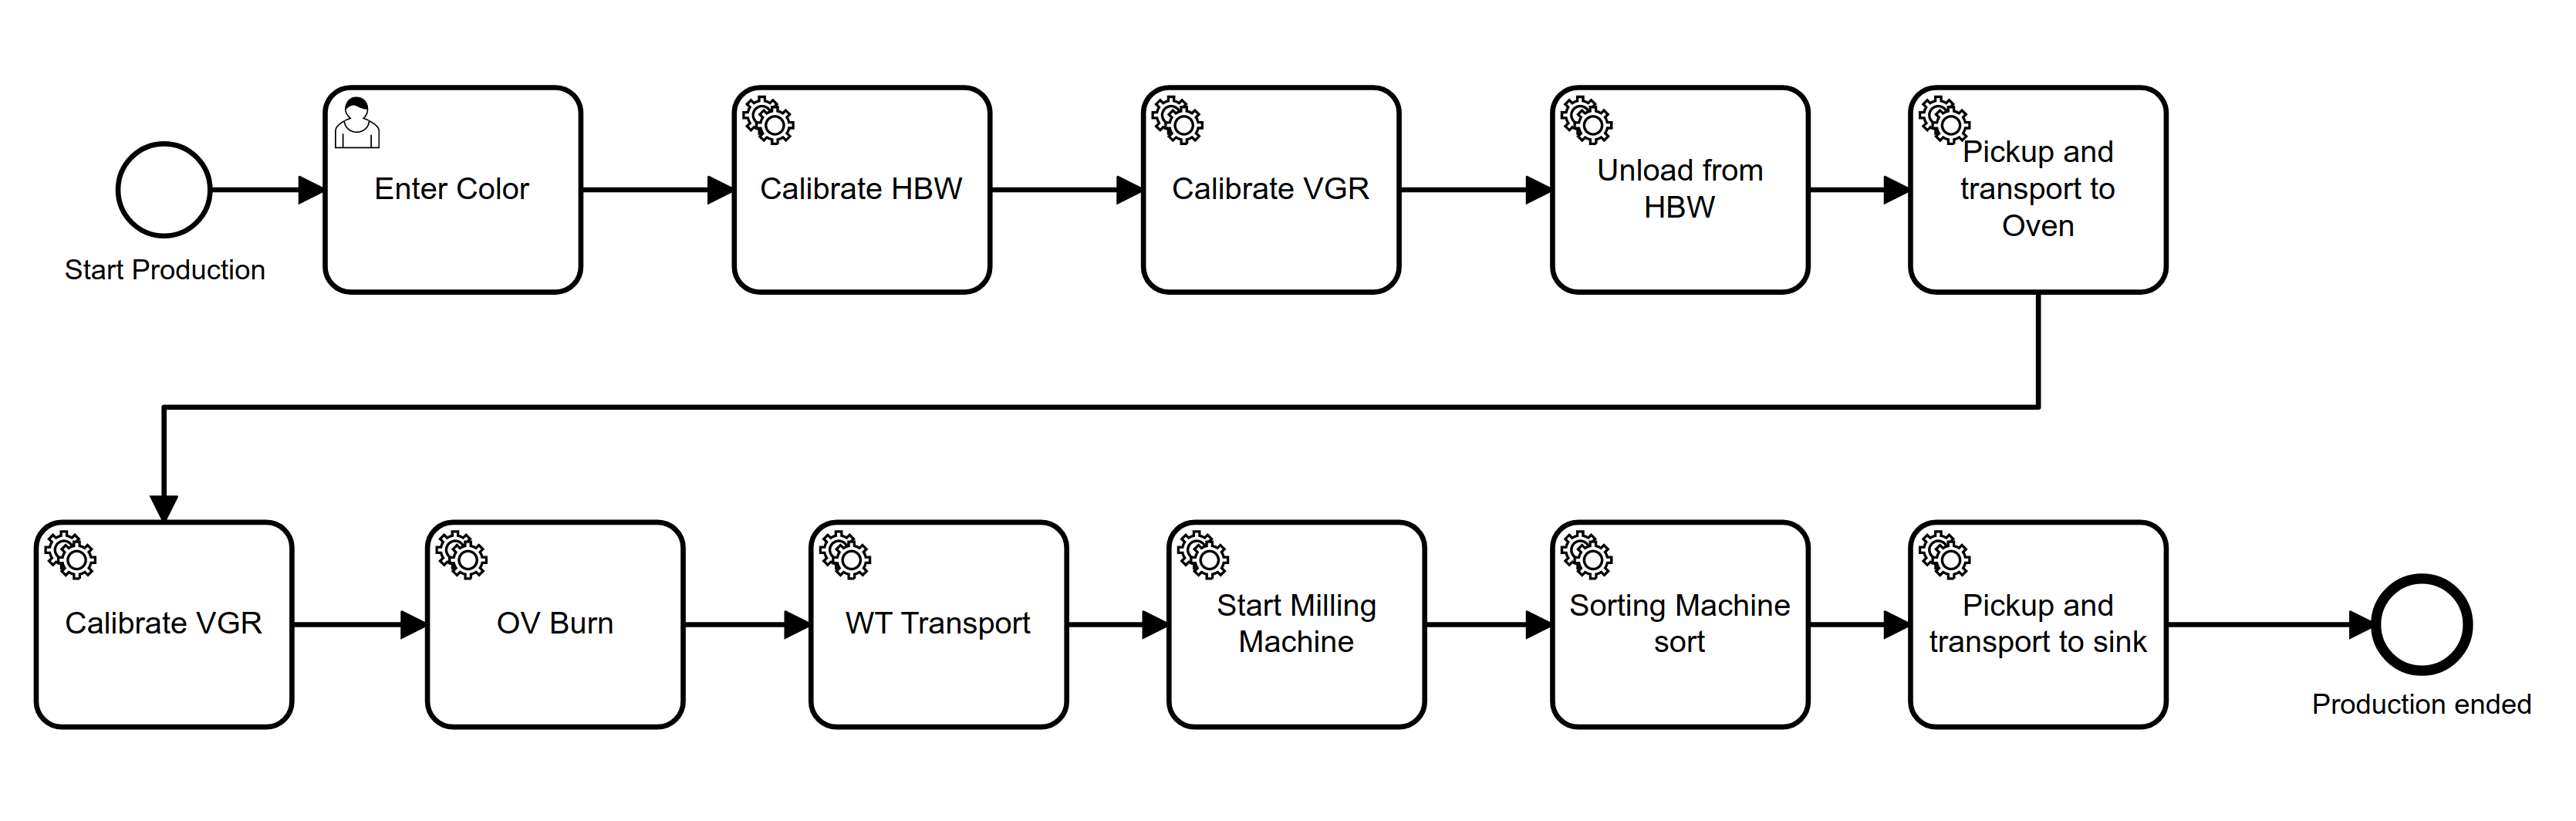
\includegraphics[width=\textwidth]{./assets/camunda_process}
    \caption{Camunda Production Process}
\end{figure}

% What we have
Even though there are no software tests available, multiple business processes, using the BPMN representation, have already been implemented for the present software system. These representations are stored in \emph{.bmpn} files are can be executed by the Camunda Modeler. This then allows the automation of the said processes.  For the testing, one particular process has been chosen to reflect the software system. It is a process that simulates production and its file is named \emph{production\_process.bpmn}. Using this file, we are able to simulate an entire production process that includes all components of the factory and hence can cover a major part of the software system. Using the contents of this file, the Camunda Modeler is able to sequentially do predetermined HTTP requests, which otherwise would have been done manually. Performing these requests manually would not only be very tedious, but also takes away standardization with a risk of making mistakes. In addition, the BPMN notation used by Camunda Modeler allows us to visually inspect at which part of the process one currently is when running it. This is an exceptionally useful feature, when trying to find out where a current issue might be located, if the visual tests fail.


% Gherkin Explanation
Gherkin on the other hand is not a software application. Instead, it is a language that is oftentimes used in conjunction with software. Hereby, one can formulate behavior in the form of specifications written in plain text and understandable by humans (\cite{cucumber-reference}). It uses a set of special keywords that enables formulating these specifications in a structured way. We can then validate whether the software does what the specifications say. This validation is primarily done with corresponding software tools. However, in our case this will be done manually. Consequently, by using the gherkin language, we are able to objectively check whether the current codebase still fulfills the specification in a form that is both human-readable and can also be routinely repeated in a standardized way.  Furthermore, the specific syntax of the Gherkin language, enables us to write objective statements.

\newpage
\myparagraph{Gherkin Framework applied to Production Process }
\begin{figure}[H]
	\centering
    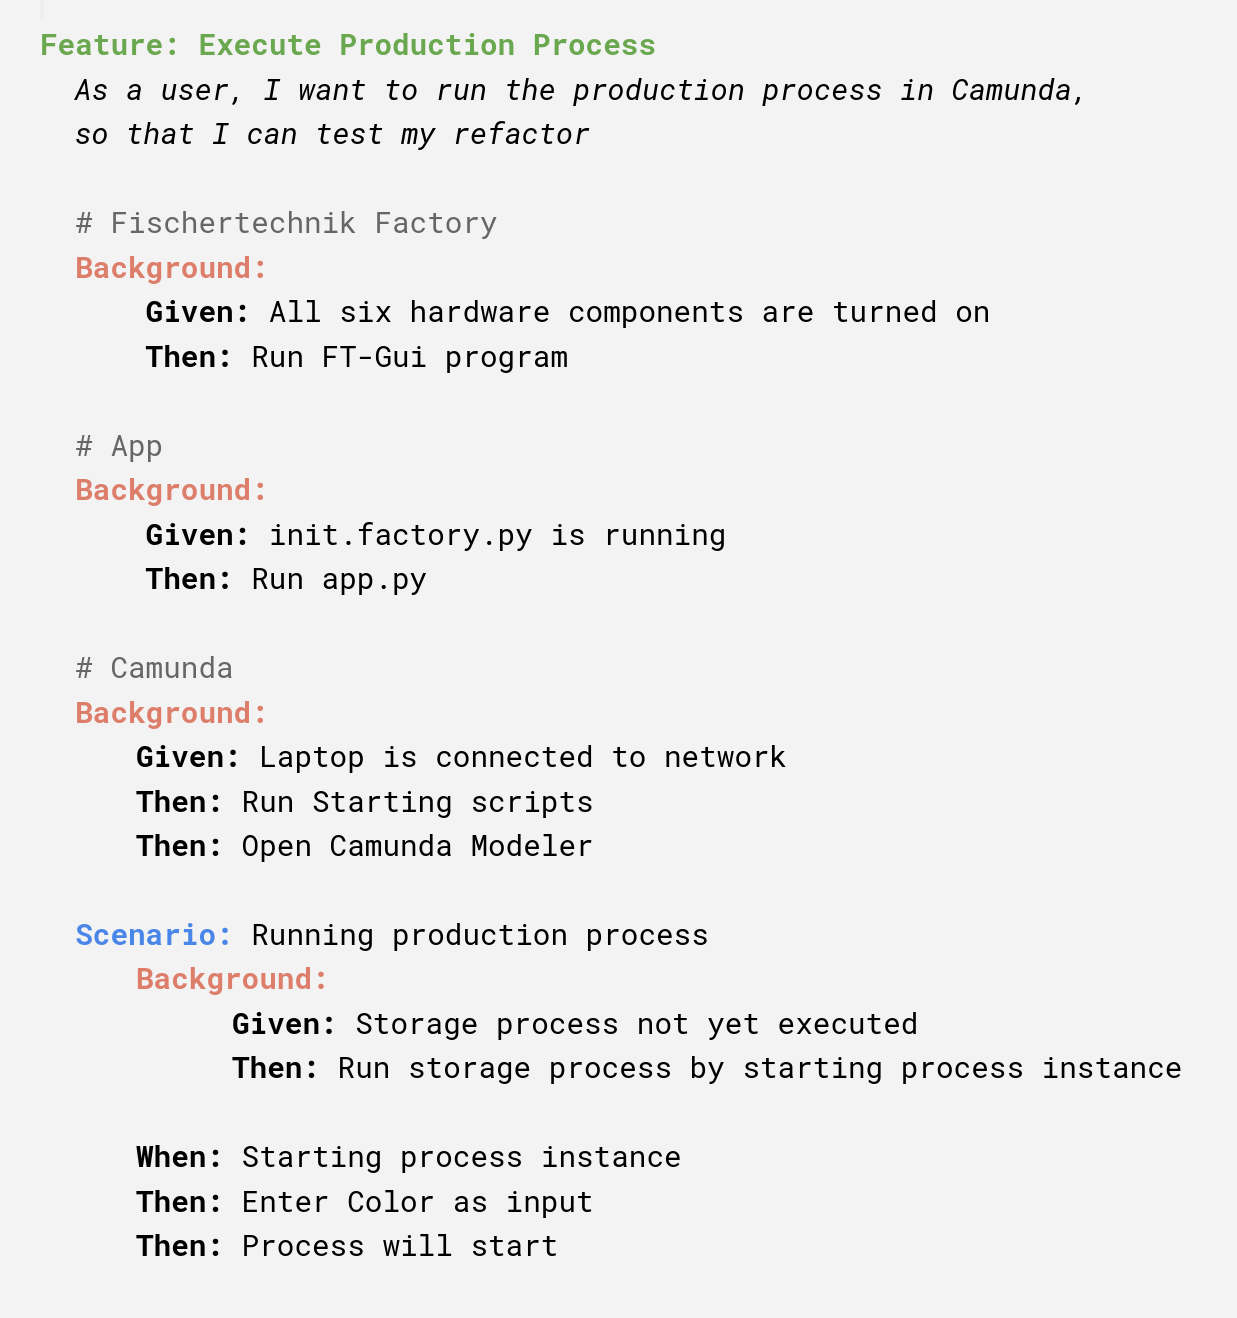
\includegraphics[width=\textwidth]{./assets/gherkin_border}
\end{figure}

As seen in the specifications above, one can observe multiple prerequisites that are necessary due to having hardware. This amount of detail is critical when wanting to reproduce this process at a later time. Even though, some specifications might seem self-evident, only then we can diminish the ambiguity associated with testing CPS. Each step must start with one of the Gherkin predefined keywords \emph{Given, When, Then, And, or But} providing the necessary structure. Such structure enables to formulate requirements that can translate to preconditions, user actions, and outcomes of the procedure.

% Optional: DEBUGGING
% - Previous stated tool is what we use to periodically check AFTER we did refactoring
% - There are preventative measure one can take DURING the refactoring. For instance bugs can be caught by trying to run python code, and see whether errors are raised
% - At current time, a lot of issues can be caught during programming itself with modern IDEs
% - With an IDE (Integrated Development Environment) Formatters and static type checkers are also able to catch bugs in the code writing process. 
% - During programming I use the pyright server as a static type checker
% - In order to early detect errors before program execution
% - Advantage is that we do not need to tediously run code all the time, but can catch them before running.
% - Don't need to run code to see malfunctions within the code
% - No errors obviously do not mean that there are no bugs. There could still be unexpected behavior.
% 	-> This is especially the case with python (statically typed language, polymorphism) == Means debugging alone would not suffice, testing is key



\section{Measuring Improvement}
% Transition
Having incorporated testing in our refactoring model, we are now in a position to consider methods for measuring the improvement of code quality after refactoring. As mentioned in the theoretical framework, to measure the internal quality, programmers can consider quality attributes as measurement criteria.

\subsection{Importance}

% Importance of tracking
Measuring improvement in code quality, allows us to evaluate how successful refactoring was. In particular, we can measure the extent of improvement, by comparing the refactored software system with its state prior to the refactoring. Having measurements aids us in making decisions in the future. If the metrics are sufficiently accurate, one could argue when to initiate and when to stop refactoring, by using them as indicators.  The comparison of the initial and final state of a refactoring can be further extended by periodically measuring code quality. We then are able to individually attribute the improvement by getting rid of specific smells. 

% Index
In order to make quantifiable measurements, the thesis employs the maintainability index, which measures how maintainable the source code is.  This measure has been chosen primarily, as it offers single-valued quantification of code quality, while considering multiple aspects of the code. A more detailed account of the index will be given in the following section.

\subsection{Maintainability Index}
or
% Introduction
For the computation of the maintainability index, the python package Radon was used. Apart from the maintainability index, this software tool is able to compute raw metrics (SLOC, comment lines, blank lines), Cyclomatic complexity and Halstead volume. These listed metrics are all interconnected, as the maintainability index in fact include all of these in its computation. The documentation of the software Radon provides brief explanations of the index and its implementation. The following section makes extensive use of the documentation in order to provide an overview (\cite{radon}). To begin, one should look at the components of the formula of this index to better understand what it wants to achieve.  


Original Formula:
\begin{equation}
\mathrm{MI}=171-5.2 \ln \mathrm{V}-0.23 \mathrm{G}-16.2 \ln \mathrm{L}
\end{equation}

\begin{itemize}
\item V = Halstead Volume
\item G = Cyclomatic Complexity
\item L = Source Lines of Code (SLOC)
\end{itemize}

Derivative (used by Radon):

\begin{equation}
\mathrm{MI}=\max \left[0,100 \frac{171-5.2 \ln \mathrm{V}-0.23 \mathrm{G}-16.2 \ln \mathrm{L}+50 \sin (\sqrt{2.4 \mathrm{C}}))}{171}\right]
\end{equation

Both formulas calculate the maintainability as a factored equation consisting of three primary components. Halstead volume is measured by multiplying halstead length (number of operators and operands) with vocabulary (number of unique operators + unique operands), Cyclomatic Complexity calculates the number of linearly independent paths in the source code, indicating the complexity of a program. SLOC counts the number of lines in the computer program.

The original equation is included as it makes it easier to understand how the individual components contribute to the end result. The second formula, which is used by Radon, is a derivative of the original formula. It is preffered as it is able to measures the maintainability between a scale from 0 to 100. As a consequence, the computation is easier to understand, as values closer to 100 indicate better maintainability. The second difference is that this formula also takes into account the percentage of commented lines indicated by the variable \emph{C}. It diminishes the significance SLOC, when the source code contains a lot of commented lines. Altough not specifically mentioned in the documentation, this is presumably the reason why Radon included this additional variable. 

\subsection{Methods used for taking measurements}

% Challenges
The method of taking measurements is also a design decision that was consciously carried out. At first, periodically taking the measurements manually was considered as a suitable method. Still after some consideration it was evident that an automated approach is more appropriate. One of the reasons was that manually running the software tool after each change quickly becomes tedious. Considerable amount of time would be spent for something that is easily automated. There would also be no clear indication on the right amount of measurments to take in a routinized way. By manually making too many measurements not only a lot of time is required, but also it would be difficult to differentiate between the individual measurements. Conversly, by having too few measurements, there would not be sufficient information available to make meaningful conclusions.

% Git hook
Regarding the timing of the measurements, it was immediately clear measuring after each commit in the version control program would be suitable. That way each measurement could directly be attributed to each commit, which includes information on code changes, such as a commit message and the possiblity to check the difference to the previous state of the prgam. Fortunately enough there exists an intuitive way to run scripts in conjunction with git activities. These types of scripts are called \emph{git hooks} or simply \emph{hooks}. As a result a hook was written using bash, implemented in a way that it is executed prior to each git commit. Consequently, this approach solved both concerns of time inefficiency and lack of attribution. It is important to note however, that this was only possible due to Radon being a command line utility. If graphical software would have been used, only a manual approach would have been feasible, if not directly implemented by the software itself. 

% Features
The bash script performs two distinct functions: computing and saving. Initially it executes radon to compute the maintainability index and including its subcomponents. Here, the result is temporarily saved in a variable. Next, these computations are then saved by writing them to a file. This file is saved locally on the computer, named after the date and time of execution. This allows the previously indicated attribution between measurement and commit. 

% Zoom
What is special about this methodology is that it enables continuous tracking in three dimensions. First, we are able to attribute individual refactoring steps in the form of commits. Second, we are able to more broadly connect measurements to the refactoring of individual code smells, preferably by indicating smells in commit messages. Lastly, by comparing current measurements to the initial state of the project, we can evaluate the overall progress since starting the refactor.

% % CONCLUSION

% % Reasons for chosing it
% - According to the issues, the methodological part of this part should in practice be more extended in order to achieve more meaningful measurements.
% - Maintainability Index is Able to measured on a file-per-file basis.
% - Because it is one index that includes a variety of indeces (to better estimate the overall maintainability)
% - Misconsception that the more advanced the programmer, the more complex the code will be. However, advanced programmers should strive to produce the simplest, elegant and easy to read programs that will achieve the objective with the least amount of steps.
% - New features request are keep coming and we are adding new code to the code base. The code base grows exponentially. 
% - The author  do  not  claim  that  the  the  MI  is  the  only  model  for  predicting  maintainability,  nordo  we  claim  it  is  the  best  overall.  
% - Chosen because of on the one hand is simple (One Value), and on the other hand measures a lot of things
% 	-> Measuring more broadly allows not to fall into the trap of self fulfilling prophecy
% 	-> This trap is apparent in the readability rating (but we are aware of it)

% % Reasons for extending to more metrics
% - It is very good that with one metric we are able to have a lot of characteristics that fit very well for the thesis
% - There are however a lot of of downsides for this especial metric, which resulted in some criticism of this metric
% - The maintainability metric should not be taken into account as seriously as a more comprehensive selection that takes into acocunt the conditions for a specific software system

% - List Shortcoming from articles
% 	-> Some of the shortcomings to be noted include
% 		-> Lack of explanation on the weights

% - The point of this study is not to optimize the metrics but to improve the internal state, these metrics are ultimately just a means of reflection / accountability.
% - Metric does not directly measure the code smells (only in part)
% - The above described methods apply much better if a whole team is refactoring a multitude of smells over a longer period of time

% Justification
% - In addition, one of the most important metrics is getting rid of code smells. The amount of code smells reduced, will mean the amount of internal problems solved.
% - This methodAccording to the issues, the methodological part of this part should in practice be more extended in order to achieve more meaningful measurements.

% How the measurements are taken is also a design decision that was taken (bewusst). First, taking the measurements manually after some time deemed approprate. After some consideration however an automated approach was deemed more appropriate. Reasons for this choice included ... however does allow us to not rely on getting rid of code smells alone as a measurement of success, but using the quality attributes.
% - An example for this false perceived notion, eliminating a large class, that however makes the code more difficult to understand, is a downgrade

% - From the individual parts of the refactoring process, this part would need the most work. Due to the fact that it doesn't directly infuence the quality of the refactoring its not that big of a problem.
% - It however as argued in the beginning of the chapter can not be left out / ignored and is thus despite its shortcomings still included. Can serve as an illustration.
% - Therefore, all in all, these methods of measurement show to be promising and especially meet our demands very well.


\section{Next steps}
[Here it could be useful to recap this chapter with a short conclusion]



% \subsection{Limitations}
% - Recap this chapter with a conclusion
% - How this detailed preparation of refactoring is important, compared to when just entering it
% - In practice not this comprehensive, but most is developed over time as an intuition through experience
% - It is however advantageous to formulate it down, making us able to discuss the topic and develop an optimal strategy
